\documentclass[CJK]{beamer}
%\usepackage{CJKutf8}
\usepackage{beamerthemesplit}
\usepackage{}
%\usetheme{Frankfurt}
%\usetheme{CambridgeUS}
%\usecolortheme{beaver}
%\usetheme{AnnArbor}
\usetheme{Dresden}
%\usebeamercolor{beetle}
\usepackage{xeCJK}
\setCJKmainfont{AR PL KaitiM GB}
%\useoutertheme{miniframes}
\usepackage{amsmath}
\usepackage{graphicx}
\usepackage{float} 
\usepackage{subfigure}
\usepackage{amssymb}
\usepackage{graphicx}
\usepackage{eufrak}
\usepackage{color}
\usepackage{array}
\usepackage{slashed}
\usepackage{simplewick}
\usepackage{tikz}
\usepackage{tcolorbox}
\usepackage[T1]{fontenc}
\graphicspath{{../figures/}}

%%figures
\def\lfig#1#2{\includegraphics[width=#1 in]{#2}}
\def\addfig#1#2{\begin{center}\includegraphics[width=#1 in]{#2}\end{center}}
\def\wulian{
\includegraphics[width=0.18in]{emoji_wulian.jpg}}
\def\bigwulian{
\includegraphics[width=0.35in]{emoji_wulian.jpg}}
\def\bye{
\includegraphics[width=0.18in]{emoji_bye.jpg}}
\def\bigbye{
\includegraphics[width=0.35in]{emoji_bye.jpg}}
\def\huaixiao{
\includegraphics[width=0.18in]{emoji_huaixiao.jpg}}
\def\bighuaixiao{
\includegraphics[width=0.35in]{emoji_huaixiao.jpg}}
\def\jianxiao{
\includegraphics[width=0.18in]{emoji_jianxiao.jpg}}
\def\bigjianxiao{
\includegraphics[width=0.35in]{emoji_jianxiao.jpg}}
%% colors
\def\blacktext#1{{\color{black}#1}}
\def\bluetext#1{{\color{blue}#1}}
\def\redtext#1{{\color{red}#1}}
\def\darkbluetext#1{{\color[rgb]{0,0.2,0.6}#1}}
\def\skybluetext#1{{\color[rgb]{0.2,0.7,1.}#1}}
\def\cyantext#1{{\color[rgb]{0.,0.5,0.5}#1}}
\def\greentext#1{{\color[rgb]{0,0.7,0.1}#1}}
\def\darkgray{\color[rgb]{0.2,0.2,0.2}}
\def\lightgray{\color[rgb]{0.6,0.6,0.6}}
\def\gray{\color[rgb]{0.4,0.4,0.4}}
\def\blue{\color{blue}}
\def\red{\color{red}}
\def\green{\color{green}}
\def\darkgreen{\color[rgb]{0,0.4,0.1}}
\def\darkblue{\color[rgb]{0,0.2,0.6}}
\def\skyblue{\color[rgb]{0.2,0.7,1.}}
%%control
\def\be{\begin{equation}}
\def\ee{\nonumber\end{equation}}
\def\bea{\begin{eqnarray*}}
\def\eea{\nonumber\end{eqnarray*}}
\def\bch{}
\def\ech{}
\def\bitem{\begin{itemize}}
\def\eitem{\end{itemize}}
\def\bcenter{\begin{center}}
\def\ecenter{\end{center}}
\def\bex{\begin{minipage}{0.2\textwidth}
\includegraphics[width=0.6in]{jugelizi.png}\end{minipage}\begin{minipage}{0.76\textwidth}}
\def\eex{\end{minipage}}
\def\chtitle#1{\frametitle{\bch#1\ech}}
\def\bmat#1{\left(\begin{array}{#1}}
\def\emat{\end{array}\right)}
\def\bcase#1{\left\{\begin{array}{#1}}
\def\ecase{\end{array}\right.}
\def\bmini#1{\begin{minipage}{#1\textwidth}}
\def\emini{\end{minipage}}
\def\tbox#1{\begin{tcolorbox}#1\end{tcolorbox}}
\def\pfrac#1#2#3{\left(\frac{\partial #1}{\partial #2}\right)_{#3}}
%%symbols
\def\bropt{\,(\ \ \ )}
\def\sone{$\star$}
\def\stwo{$\star\star$}
\def\sthree{$\star\star\star$}
\def\sfour{$\star\star\star\star$}
\def\sfive{$\star\star\star\star\star$}
\def\rint{{\int_\leftrightarrow}}
\def\roint{{\oint_\leftrightarrow}}
\def\stdHf{{\textit{\r H}_f}}
\def\deltaH{{\Delta \textit{\r H}}}
\def\ii{{\dot{\imath}}}
\def\skipline{{\vskip0.1in}}
\def\skiplines{{\vskip0.2in}}
\def\lagr{{\mathcal{L}}}
\def\hamil{{\mathcal{H}}}
\def\vecv{{\mathbf{v}}}
\def\vecx{{\mathbf{x}}}
\def\vecy{{\mathbf{y}}}
\def\veck{{\mathbf{k}}}
\def\vecp{{\mathbf{p}}}
\def\vecn{{\mathbf{n}}}
\def\vecA{{\mathbf{A}}}
\def\vecP{{\mathbf{P}}}
\def\vecsigma{{\mathbf{\sigma}}}
\def\hatJn{{\hat{J_\vecn}}}
\def\hatJx{{\hat{J_x}}}
\def\hatJy{{\hat{J_y}}}
\def\hatJz{{\hat{J_z}}}
\def\hatj#1{\hat{J_{#1}}}
\def\hatphi{{\hat{\phi}}}
\def\hatq{{\hat{q}}}
\def\hatpi{{\hat{\pi}}}
\def\vel{\upsilon}
\def\Dint{{\mathcal{D}}}
\def\adag{{\hat{a}^\dagger}}
\def\bdag{{\hat{b}^\dagger}}
\def\cdag{{\hat{c}^\dagger}}
\def\ddag{{\hat{d}^\dagger}}
\def\hata{{\hat{a}}}
\def\hatb{{\hat{b}}}
\def\hatc{{\hat{c}}}
\def\hatd{{\hat{d}}}
\def\hatN{{\hat{N}}}
\def\hatH{{\hat{H}}}
\def\hatp{{\hat{p}}}
\def\Fup{{F^{\mu\nu}}}
\def\Fdown{{F_{\mu\nu}}}
\def\newl{\nonumber \\}
\def\vece{\mathrm{e}}
\def\calM{{\mathcal{M}}}
\def\calT{{\mathcal{T}}}
\def\calR{{\mathcal{R}}}
\def\barpsi{\bar{\psi}}
\def\baru{\bar{u}}
\def\barv{\bar{\upsilon}}
\def\qeq{\stackrel{?}{=}}
\def\torder#1{\mathcal{T}\left(#1\right)}
\def\rorder#1{\mathcal{R}\left(#1\right)}
\def\contr#1#2{\contraction{}{#1}{}{#2}#1#2}
\def\trof#1{\mathrm{Tr}\left(#1\right)}
\def\trace{\mathrm{Tr}}
\def\comm#1{\ \ \ \left(\mathrm{used}\ #1\right)}
\def\tcomm#1{\ \ \ (\text{#1})}
\def\slp{\slashed{p}}
\def\slk{\slashed{k}}
\def\calp{{\mathfrak{p}}}
\def\veccalp{\mathbf{\mathfrak{p}}}
\def\Tthree{T_{\tiny \textcircled{3}}}
\def\pthree{p_{\tiny \textcircled{3}}}
\def\dbar{{\,\mathchar'26\mkern-12mu d}}
\def\erf{\mathrm{erf}}
\def\const{\mathrm{constant}}
\def\pheat{\pfrac p{\ln T}V}
\def\vheat{\pfrac V{\ln T}p}
%%units
\def\fdeg{{^\circ \mathrm{F}}}
\def\cdeg{^\circ \mathrm{C}}
\def\atm{\,\mathrm{atm}}
\def\angstrom{\,\text{\AA}}
\def\SIL{\,\mathrm{L}}
\def\SIkm{\,\mathrm{km}}
\def\SIyr{\,\mathrm{yr}}
\def\SIGyr{\,\mathrm{Gyr}}
\def\SIV{\,\mathrm{V}}
\def\SImV{\,\mathrm{mV}}
\def\SIeV{\,\mathrm{eV}}
\def\SIkeV{\,\mathrm{keV}}
\def\SIMeV{\,\mathrm{MeV}}
\def\SIGeV{\,\mathrm{GeV}}
\def\SIcal{\,\mathrm{cal}}
\def\SIkcal{\,\mathrm{kcal}}
\def\SImol{\,\mathrm{mol}}
\def\SIN{\,\mathrm{N}}
\def\SIHz{\,\mathrm{Hz}}
\def\SIm{\,\mathrm{m}}
\def\SIcm{\,\mathrm{cm}}
\def\SIfm{\,\mathrm{fm}}
\def\SImm{\,\mathrm{mm}}
\def\SInm{\,\mathrm{nm}}
\def\SImum{\,\mathrm{\mu m}}
\def\SIJ{\,\mathrm{J}}
\def\SIW{\,\mathrm{W}}
\def\SIkJ{\,\mathrm{kJ}}
\def\SIs{\,\mathrm{s}}
\def\SIkg{\,\mathrm{kg}}
\def\SIg{\,\mathrm{g}}
\def\SIK{\,\mathrm{K}}
\def\SImmHg{\,\mathrm{mmHg}}
\def\SIPa{\,\mathrm{Pa}}
\def\secpage#1#2{\begin{frame}\bch\bcenter{\bf \Huge #1} \skipline \tbox{\bcenter #2\ecenter}\ecenter\ech\end{frame}}

\usepackage{amssymb}
\newcommand{\field}{\mathscr{F}}

\newcommand{\reals}{\mathbb{R}}
\newcommand{\complexs}{\mathbb{C}}
\newcommand{\ints}{\mathbb{Z}}
%\newcommand{\dim}{\mathrm{dim\ }}
\newcommand{\diag}{\mathrm{diag \ }}
\newcommand{\up}{\uparrow}
\newcommand{\down}{\downarrow}
\newcommand{\su}{\mathfrak{su}}
\newcommand{\so}{\mathfrak{so}}
\newcommand{\tr}{\mathrm{tr\ }}
\newcommand{\card}{\mathrm{card \ }}
\newcommand{\spa}{\,\,\,}
\newcommand{\lag}{\mathcal{L}}
\newtheorem{thm}{引理}[section]
\newtheorem{axm}{公理}[section]
\newtheorem{dfn}{定义}[section]

%\cpic{<尺寸>}{<文件名>}}用于生成居中的图片。
\newcommand{\cpic}[2]{
\begin{center}
\includegraphics[scale=#1]{#2}
\end{center}
}

%\cpicn{<尺寸>}{<文件名>}{<注释>}用于生成居中且带有注释的图片,其label为图片名。
\newcommand{\cpicn}[3]
{
\begin{figure}[h!]
\cpic{#1}{#2}
\caption{#3\label{#2}}
\end{figure}
}

\title{AQM Talk 12 Representing Relativistic Quantum State}
  \author{}
  \date{}


\begin{document}

\begin{frame}
 
\begin{center}
\begin{Large}
  \bch
{\bf A}dvanced {\bf Q}uantum {\bf M}echanics

{\vskip 0.1in}

Talk 12 Representing Relativistic Quantum State
\ech
\end{Large}
\end{center}


\vskip 0.1in
\begin{center}
Haoting Xu
\vskip 0.1in
xuht9@mail2.sysu.edu.cn
\vskip 0.1in
{\tiny \url{https://github.com/HaotingXu/seminar_lec} }\\
\end{center}


\end{frame}
\section{Tensor Notation}
\begin{frame}\frametitle{\bch自然单位制\ech}
  \be
  c = \hbar =1
  \ee
\end{frame}
\begin{frame}\frametitle{\bch 4-矢量和度规\ech}
  \bch
  四矢量的逆变分量为
  \be
  A = \left(A^{\mu}\right) = \left(A^0,\vec{A}\right)
  \ee
  注意,拉丁指标$i,j,k$从$1$取到$3$,希腊指标$\alpha,\beta,\gamma$从$0$取到$3$。4-位置矢量为
  \be
  x = \left(t,x,y,z\right)
  \ee
  Minkowski 度规
  \be
  g = \left(g_{\mu\nu}\right) = \mathrm{diag}(1,-1,-1,-1)
  \ee
  定义
  \be
  g^{-1} = \left(g^{\mu\nu}\right) = \mathrm{diag}(1,-1,-1,-1)
  \ee
  \ech
\end{frame}
\begin{frame}\frametitle{\bch 内积和Minkowski 时空\ech}
  \bch
  指标升降规则
  \be
  A_\mu = g_{\mu\nu}A^{\nu},\, T_{\mu\nu} = g_{\mu\lambda}g_{\nu \omega} T^{\lambda \omega}
  \ee
  定义内积
  \be
  g\left(A,B\right) = g_{\mu\nu} A^{\mu}B^{\nu} = A_\mu B^{\mu}
  \ee
  4-矢量长度为
  \be
  A^2 = \left(A^0\right)^2 - \vec{A}^2
  \ee
  如果$A^2>0$,则称$A$为类时的,如果$A^2>0$,称$A$为类空的。特殊地,对于4-位置矢量
  \be
  x^2 = t^2 - x^2-y^2 - z^2
  \ee
  定义Minkowski 时空为$M = (\mathbb{R}^4,g)$
  \ech
\end{frame}
\begin{frame}\frametitle{Levi-Civita tensor}
  \bch
  引入三维 Levi-Civita 张量$\epsilon_{ijk} = \epsilon^{ijk}$,它满足
  \bea
  \epsilon^{ijk}\epsilon^{ijk} &=& 6\\
  \epsilon^{ijk}\epsilon^{klm} &=& \delta^{il}\delta^{jm} - \delta^{im}\delta^{jl}\\
  \epsilon^{ijk}\epsilon^{lmn} &=& \delta^{il}\left(\delta^{jm}\delta^{kn} - \delta^{jn}\delta^{km}\right)-\delta^{im}\left(\delta^{jl}\delta^{kn} - \delta^{jn}\delta^{kl}\right)\\
  & &+\delta^{in}\left(\delta^{jl}\delta^{km} - \delta^{jm}\delta^{kl}\right)
  \eea
  \ech
\end{frame}
\begin{frame}\frametitle{Levi-Civita tensor}
  \bch
  对于四维时空,定义Levi-Civita tensor,它满足指标升降规,且有如下对应性质
  \be
  \epsilon^{\alpha \beta\gamma\delta}\epsilon_{\alpha\beta\gamma\delta} = -24
  \ee
  等等,因为后面几乎用不到,所以不抄了。
  \ech
\end{frame}
\section{Poincare group}
\begin{frame}\frametitle{\bch洛伦兹变换\ech}
  \bch
  洛伦兹变换是保内积不变的变换。假设有两个4-矢量$x,y$,经过洛伦兹变换后成为
  \be
  x^{\prime \mu} = \Lambda ^{\mu}_{\spa\nu} x^{\nu},\spa ,y^{\prime \mu} = \Lambda ^{\mu}_{\spa\nu} y^{\nu}  
  \ee
  他们的内积为
  \be
  x^{\prime \mu} y_{\mu}^{\prime} = \Lambda^{\mu}_{\spa\nu} \Lambda^{\lambda}_{\spa\mu}x^{\nu} y_{\lambda} = g_{\nu\lambda}x^{\nu}y^{\lambda}
  \ee
  进而得到洛伦兹变换应该满足的关系
  \be
  \left(\Lambda^T\right)^{\spa \mu}_{\nu} g_{\mu\omega}\Lambda^{\omega}_{\spa\lambda} = g_{\nu \lambda}
  \ee
  即
  \be
  \Lambda^T g\Lambda = g
  \ee
  \ech
\end{frame}
\begin{frame}\frametitle{\bch洛伦兹变换\ech}
  \bch
 
  例如,在狭义相对论中,两个惯性系之间的变换为
  \be
  x^{\prime} =
  \begin{pmatrix}
    \cosh \xi &-\sinh\xi&0&0\\
    -\sinh\xi& \cosh\xi& 0&0 \\
    0&0&1&0\\
    0&0&0&1
  \end{pmatrix}
  \begin{pmatrix}
    x^0 \\ x^1\\x^2\\x^3
  \end{pmatrix}
  = \Lambda^{(01)}x
  \ee
  可以验证,上面的变换$\Lambda^{(01)}$是一个洛伦兹变换。这样的变换又被叫做standard configuration Lorentz transformation,它是standard transformation(boost)的一种,系数$\xi$又被称做快度(rapidity, boost parameter)。为了和经典的伽利略变换对应起来,我们取
  \be
  \cosh\xi = \gamma , \, \sinh\xi = \beta\gamma
  \ee
  就回到我们熟悉的洛伦兹变换。
  \ech
\end{frame}
\begin{frame}\frametitle{\bch洛伦兹群\ech}
  \bch
  洛伦兹群的定义为
  \be
  \mathcal{L} = \{ \Lambda : M \rightarrow M, x^{\prime}\cdot y^{\prime} = x\cdot y, \mathrm{where} \spa x^{\prime} = \Lambda x, \spa y^{\prime} = \Lambda y\}
  \ee
  上面的条件可以等价地写成
  \be
  g = \Lambda^Tg\Lambda,\, or \spa g_{\mu\omega}\Lambda^{\mu}_{\spa\nu}\Lambda^{\omega}_{\spa\lambda} = g_{\nu\lambda}
  \ee
  对上面的条件两边求行列式,得到
  \be
  \left(\mathrm{det} \Lambda\right)^2 = 1
  \ee
  令$\nu = \lambda = 0$,得到
  \be
  \left(\Lambda^{0}_{\spa 0 }\right)^2  - \sum_{i=1}^3 \left(\Lambda^{i}_{\spa 0}\right)^2 = 1
  \ee
  因此有
  \be
  \Lambda^{0}_{\spa 0 } \ge 1 \, or\spa \Lambda^{0}_{\spa 0 }\le -1
  \ee
  \ech
\end{frame}
\begin{frame}\frametitle{\bch洛伦兹群\ech}
  \bch
  因此可以用$\det\Lambda$和$\Lambda^{0}_{\spa 0 }$的符号给洛伦兹群分类。定义
  \be
  \mathcal{L}_{+} = \{\Lambda\in \lag : \mathrm{det}\Lambda=1\},\spa \lag^{\uparrow} = \{ \Lambda\in\lag :\Lambda^{0}_{\spa 0 }\ge 1\}
  \ee
  其中$\mathcal{L}_{+}$又被叫做Pure Lorentz Group,$\lag^{\uparrow}$被叫做Orthochronous Lorentz Group。进而定义$\lag^\uparrow_+ = \lag^\uparrow\cap\lag_+$,可以证明,上面三个群都是洛伦兹群的子群。使用同样的规则,也可以定义$\lag_-^\uparrow, \lag_-^\downarrow, \lag_+^\downarrow$,它们都不是子群,通过下面的变换,可以说明两个元素的乘法不在群里面。
  \begin{itemize}
  \item Parity $\Lambda_p = \diag \left(1,-1,-1,-1\right)\in \lag_-^\uparrow$
  \item Time reversal $\Lambda_T = \diag \left(-1,1,1,1\right)\in \lag_-^\downarrow$
  \item Spacetime inversion $\Lambda_{PT} = \diag \left(-1,-1,-1,-1\right)\in \lag_+^\downarrow$
  \end{itemize}
  另外,集合$\lag_0 = \lag_+^\uparrow \cap\lag_-^\downarrow$也是洛伦兹群的一个子群。
  \ech
\end{frame}
\begin{frame}\frametitle{\bch洛伦兹群\ech}
  \bch
  通过上面的变换,我们可以将$\lag_-^\uparrow, \lag_-^\downarrow, \lag_+^\downarrow$三个子群映射到pure and orthochronous Lorentz Group中
  \be
  \lag = \lag_+^\uparrow \cup\lag_-^\uparrow\cup \lag_-^\downarrow\cup \lag_+^\downarrow = \lag_+^\uparrow\cup \Lambda_P\lag_+^\uparrow\cup\Lambda_T\lag_+^\uparrow\cup \Lambda_{PT}\lag_+^\uparrow
  \ee
  \cpicn{0.3}{subgroup}{洛伦兹群的子群}
  \ech
\end{frame}
\begin{frame}\frametitle{\bch洛伦兹群\ech}
  \bch
  所以我们现在只需要来研究$\lag_+^\uparrow$,这个子群又被叫做$SO^{+}(1,3)$群,它是一个李群。因此有
  \be
  \Lambda = \exp\left(-\frac{i}{2} \omega_{\mu\nu} M^{\mu\nu}\right)
  \ee
  其中$M^{\mu\nu}$为生成元,其中指标$\mu\nu$为生成元矩阵的编号。不妨设$M^{\mu\nu} = -M^{\nu\mu}$。注意这和我们熟悉的$SO(N)$群不同,在那里生成元矩阵是反称的,那是因为它满足$R^TR = 1$,而这里$\Lambda$却满足$\Lambda^T g\Lambda = g$,将无穷小变换带入这个关系式,将得到
  \be
  g_{\nu\omega}M^{\omega}_{\spa \lambda} + g_{\mu\lambda}M^{\mu}_{\spa\nu}=0
  \ee
  上面这个关系式保证了生成元有六个独立分量,但是不一定反对称,因此有六个独立的生成元矩阵。
  \ech
\end{frame}
\begin{frame}\frametitle{\bch 洛伦兹群的生成元\ech}
  \bch
  生成元有多种取法,我们取$M^{\mu\nu}$就对应与无穷小的$\Lambda^{\mu\nu}$使得$\Lambda^{\mu\nu} \simeq 1-\frac{i}{2} M^{\mu\nu}$现在对于无穷小standard configuration Lorentz transformation,我们求解它的生成元
  \be
  M^{01} = i\frac{d\Lambda(\xi)}{d\xi}\vert_{\xi = 0} =
  \begin{pmatrix}
    0 &-i&0&0\\
    -i &0&0&0\\
    0 &0&0&0\\
    0 &0&0&0
  \end{pmatrix}
  \ee
  可见,$M^{0i}$对应与Lorentz boost,而$M^{ij}$对应于三维空间的转动。
  \ech
\end{frame}

\begin{frame}\frametitle{\bch洛伦兹群的生成元\ech}
  \bch
  因此,可以将反对称的生成元$M^{\mu\nu}$拆分成$J^i,K^i$,$2\times 3=6$个矩阵,它们与生成元的关系为
  \be
  J^i = -\frac{1}{2} \epsilon^{ijk} M^{jk} ,\, K^i = M^{0i}
  \ee
  可以证明,它们满足对易关系
  \bea
  \left[J^i,J^j\right]&=&i\epsilon^{ijk}J^k\\
  \left[J^i,K^j\right]&=&i\epsilon^{ijk}K^k\\
  \left[K^i,K^j\right]&=&-i\epsilon^{ijk}J^k
  \eea
  可见,它们形成了一个李代数。为了好看,我们定义
  \bea
  \vec{j} &=& \frac{1}{2}\left(\vec{J}+i\vec{K}\right)\\
  \vec{k} &=& \frac{1}{2}\left(\vec{J}-i\vec{K}\right)
  \eea
  
  \ech
\end{frame}
\begin{frame}\frametitle{\bch洛伦兹代数\ech}
  \bch
  这时对易关系变为
  \bea
  \left[j^i,j^j\right]&=&i\epsilon^{ijk}j^k\\
  \left[j^i,k^j\right]&=&0\\
  \left[k^i,k^j\right]&=&i\epsilon^{ijk}k^k
  \eea
  我们说,$\vec{j},\vec{k}$是脱耦的。我们将上述李代数的结构叫做洛伦兹代数,记作$\su (2) \oplus \su (2)$。对应的洛伦兹群的表示为$D^j\otimes D^{j^{\prime}}$, $D^j$是$SU(2)$的不可约表示。我们将$D^j$在$|j,m\rangle$这组基下展开,那么洛伦兹群的基为
  \be
  |j,m;j^{\prime},m^{\prime}\rangle = |j,m\rangle |j^{\prime},m^{\prime}\rangle
  \ee
  例如,$D^{\left(\frac{1}{2},0\right)}$和$D^{0,\left(\frac{1}{2}\right)}$的生成元的表示为
  \be
  \vec{j} = \frac{1}{2}\vec{\sigma},\,\vec{k}=0 \, \spa \mathrm{and} \spa \vec{j} = 0,\, \vec{k} = \frac{1}{2}\vec{\sigma}
  \ee
  其中$\vec{\sigma}$为三个泡利矩阵。
  \ech
\end{frame}
\begin{frame}\frametitle{\bch Poincare 群\ech}
  \bch
  Poincare群的定义为
  \be
  \mathcal{P} = \{\left(\Lambda, a \right):x^\mu\rightarrow x^{\prime\mu} = \Lambda^\mu_\nu x^\nu+ a^{\mu}\}
  \ee
  其中$\Lambda \in \lag $是一个洛伦兹变换,$a\in \mathbb{R}^4$是一个Lorentz Translation。如果$P_+^{\uparrow}$是一个pure and orthochronous Pioncare Group,如果$\Lambda \in \lag_+^{\uparrow}$。可以得到两个群的乘法为
  \be
  \left(\Lambda_2,a_2\right)\left(\Lambda_1,a_1\right) = \left(\Lambda_2\Lambda_1,\, \Lambda_2a_1+a_2\right)
  \ee
  显然Poincare群有一个五维表示
  \be
  \begin{pmatrix}
    \Lambda &a \\
    0&1
  \end{pmatrix}
  _{5\times 5}
  \ee
  Poincare群的逆为$\left(\Lambda^{-1},-\Lambda^{-1}a\right)$。
  \ech
\end{frame}
\begin{frame}\frametitle{\bch Poincare群的生成元\ech}
  \bch
  我们已经知道了洛伦兹群的生成元
  \be
  U\left(\Lambda,0\right) = \exp \left(-\frac{i}{2} \omega_{\mu\nu} M^{\mu\nu}\right)
  \ee
  我们再来看poincare translation的生成元即$U\left(1,a\right)$的生成元。我们思考一下可以发现生成元只有对角项,所以生成元只有四个,因此
  \be
  U\left(1,a\right) = \exp\left(ia_\mu P^{\mu}\right)
  \ee
  因此,如果Poincare群在一阶近似附近,那么Poincare群元可近似写为
  \be
  U\left(\Lambda,a\right) \simeq \left(-\frac{i}{2}\omega_{\mu\nu}M^{\mu\nu}+ia_\mu P^{\mu}\right)
  \ee
  \ech
\end{frame}
\begin{frame}\frametitle{\bch生成元的对易关系\ech}
  \bch
  我们再来看生成元的对易关系。使用洛伦兹群的定义,并结合$U_1U_2U_1^{-1} = 1+B+\left[A,B\right]$,我们就得到了生成元的对易关系
  \bea
  \left[M^{\mu\nu},M^{\rho\sigma}\right] &=& i\left(g^{\mu\rho}M^{\nu\sigma}+g^{\nu\sigma}M^{\mu\rho}-g^{\mu\sigma}M^{\nu\rho} - g^{\nu\rho}M^{\mu\sigma} \right)\\
  \left[M^{\mu\nu},P^\sigma\right] &=& -i\left( g^{\nu\sigma}P^{\mu} - g^{\mu\sigma}P^{\nu}\right)\\
  \left[P^\mu,P^\nu\right] &=&0
  \eea
  \ech
\end{frame}
\begin{frame}\frametitle{\bch Casimir 算符\ech}
  \bch
  Casimir算符定义为
  \begin{itemize}
  \item 是由生成元构建的。
  \item 和所有生成元对易。
  \item 是该群的不变量。
  \end{itemize}
  比如说,$\vec{J}^2$是$SO(3)$的Casimir不变量。Poincare群的Casimir算符有两个,分别为$P^2 = P_\mu P^\mu,\, w^2 = w_\mu w^\mu$。$w$被叫做Pauli-Lubanski 矢量,定义为
  \be
  w_\sigma = \frac{1}{2}\epsilon_{\sigma\mu\nu\lambda}M^{\mu\nu}P^{\lambda}
  \ee
  \ech
\end{frame}
\begin{frame}\frametitle{\bch Pauli-Lubanski矢量\ech}
  \bch
  利用Pauli- Lubanski矢量的定义,我们得到它与生成元的对易关系
  \bea
  \left[M_{\mu\nu},w_\sigma\right] &=& -i\left(g_{\nu\sigma}w_\mu - g_{\mu\sigma}w_\nu\right)\\
  \left[P_\mu,w_\nu\right] &=&0 \\
  \left[w_\mu,w_\nu\right] &=& i\epsilon_{\mu\nu\rho\sigma}w^{\rho}P^{\sigma}
  \eea
  还有一种书写Pauli-Lubanski矢量的方法
  \be
  v^{\mu\nu\rho} = P^{\mu}M^{\nu\rho}+P^{\nu}M^{\rho\mu}+P^{\rho}M^{\mu\nu}
  \ee
  则$w = \left(v^{321},v^{320},v^{310},v^{210}\right)$。$w^2$使用之前的生成元可以表示为
  \be
  w^2 = -\frac{1}{2} M^{\mu\nu}M_{\mu\nu}P^2 + M^{\mu\sigma}M_{\nu\sigma}P_\mu P^\nu
  \ee
  \ech
\end{frame}
\begin{frame}\frametitle{\bch舒尔引理\ech}
  \bch
  \begin{thm}
   (舒尔引理) 如果$U(g)$是不可约表示,并且$A$和所有的$U(g)$对易,那么$A$一定是单位算符的倍数,即$A = \alpha I$,$\alpha$是一个常数。
  \end{thm}
  \ech
\end{frame}
\section{States and Particles}
\begin{frame}\frametitle{\bch来点物理\ech}
  \bch
  上面我们讨论的都是纯数学,现在我们加点物理。我们把群的元素看成是希尔伯特空间的算符。
  \ech
\end{frame}

\begin{frame}\frametitle{\bch什么是粒子?\ech}
  \bch
  如何区分不同的粒子?在相对论中坐标变换是Poincare变换,所以每个态在Poincare变换下是不同的,但是,你知道它还是一个粒子。所以我们希望用一个Poincare变换下的不变量。什么是Poincare变换下的不变量? 根据舒尔引理,Casimir算符的本征值!
  所以我们说,我们通过{\color{blue}Poincare群不可约表示的Casimir算符来区分不同的粒子}!
  \ech
\end{frame}
\begin{frame}\frametitle{\bch Poincare群的Casimir 不变量\ech}
  \bch
  现在,我们不把Poincare变换作用的矢量选成4-位置,我们选成4-动量,即$\vec{p} = \left(E,\vec{p}\right)$,使用书中所谓的correspondence principle,生成元$P$的本征值就是$p = \left(p^{\mu}\right) = \left(E,\vec{p}\right)$,所以说$P$就是动量算符。{\color{blue} 动量算符就是Lorentz translation 的生成元!}

  我们知道,$p^2 = p_\mu p^\mu = m^2$,因此$P^2 = m^2 I$,我们知道粒子的质量$m$是一个用来区分不同粒子的指标。 
  \ech
\end{frame}
\begin{frame}\frametitle{\bch 粒子的自旋\ech}
  \bch
  我们知道还有一个Casimir 不变量,那个是$w^2$,我们来看看这是啥。我们将$w$作用在一组基$|m,p^\mu,\gamma\rangle$,简单起见,我们取$p^\mu = \left(m,\vec{0}\right)$,我们得到
  \bea
  w^0|m,p^\mu,\gamma\rangle &=& 0\\
  w^i|m,p^\mu,\gamma\rangle &=& mJ^i|m,p^\mu,\gamma\rangle
  \eea
  我们计算出了另外一个Casimir算符,它是
  \be
  w^2|m,p^\mu,\gamma\rangle = -m^2s(s+1)|m,p^\mu,\gamma\rangle
  \ee
  我们得到了另外一个区分不同粒子(态)的参数:自旋!
  \ech
\end{frame}
\begin{frame}\frametitle{\bch 描述一个粒子\ech}
  \bch
  最后,我们还需要自旋角动量在某一个轴的投影算符来描述一个态。故最后一个态可以描述为
  \be
  |m,p;s,m_S\rangle
  \ee
  $m_s$又成为螺旋性(helicity),因此常常又被记作$h$。
  \ech
\end{frame}
\begin{frame}\frametitle{\bch 粒子的分类\ech}
  \bch
  Wigner 按照$p^2$和$p_0$给粒子分了四种情况
  \begin{itemize}
  \item $p^2=m^2>0$, $p^0>0$ 或$p^0<0$ 
\includegraphics[scale=0.02]{error} 
  \item $p^2=0$, $p\ne 0$,  $p^0>0$ 或$p^0<0$ 
\includegraphics[scale=0.02]{error}
  \item $p^2=0$, $p^0= 0$ 真空 vacuum
  \item $p^2<0$ 超光子tachyons
  \end{itemize}
  \ech
\end{frame}
\begin{frame}\frametitle{\bch态如何变换\ech}
  \bch
  记
  \be
  U(a) = U(1_4, a) = \exp(ia\cdot P)
  \ee
  $P = (P^0,\vec{P})$是4-动量算符,$P^0$便是哈密顿量,在相对论情形下
  \be
  P^0 = + \sqrt{m^2 + \vec{P}^2}
  \ee
  引入平面波基矢$|p,\zeta\rangle$,使得
  \be
  P^\mu|p,\zeta\rangle = p^\mu|p,\zeta\rangle
  \ee
  $\zeta$是除了动量之外其他的量子数。于是有
  \be
  U(a) |p,\zeta\rangle = e^{ia\cdot P}|p,\zeta\rangle = e^{iap}|p,\zeta\rangle
  \ee
  \ech
\end{frame}
\begin{frame}\frametitle{\bch进行坐标变换\ech}
  \bch
  从这里开始我就看不懂了。

  (应该是)进行洛伦兹变换使得$p = \Lambda (p)p^{\prime}$,变换后新的基矢记作$|\Lambda (p),\zeta\rangle$(terrible notations),于是根据定义
  \be
  U(a)|\Lambda (p),\zeta\rangle = U(a)U(\Lambda (p))|p^{\prime},\zeta\rangle
  \ee
  利用关系({\color{red} 我无法得到的关系})
  \be
  U(a) U(\Lambda (p)) = U(\Lambda(p),a) = U(\Lambda(p)) U(\Lambda(p)^{-1}a)
  \ee
  之后的操作我就更看不懂了,例如$[\Lambda(p)^{-1}a]\cdot p^{\prime} = a\cdot \Lambda(p) p^{\prime} = a\cdot p$,最后结果为
  \be
  U(a)|\Lambda(p),\zeta\rangle = e^{ia\cdot p}|\Lambda(p),\zeta\rangle
  \ee
  最终得到
  \be
  P^\mu |\Lambda(p),\zeta\rangle = p^\mu |\Lambda(p),\zeta\rangle
  \ee
  这说明了啥?
  \ech
\end{frame}
\section{Spin}
\begin{frame}\frametitle{little group}
  \bch
  从上面可以看到,有一些Poincare变换保持$p^{\prime}$不变。我们现在来研究这些变换。记保持$p^{\prime}$不变的群为little group(or stabilizer),记作$W(p^\prime)$,因为是Wigner引入的这个小群。其中的群元记作$\Gamma \in W(p^{\prime})$。
  \cpicn{0.25}{Wigner}{\bch 还记得凝聚态物理中遇到的Wigner吗?\ech}
  \ech
\end{frame}
\begin{frame}
\frametitle{\bch 凝聚态物理复习\ech}
\bch
从左到右\par
布拉伐-Auguste Bravais,1811-1863,法国人
\par
Eugene Wigner,1902-1995,匈牙利人
\par
Frederick Seitz,1911-2008,美国人
\begin{figure}
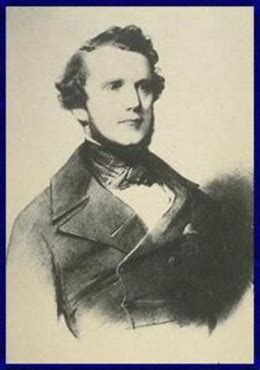
\includegraphics[scale=0.21]{bravais}
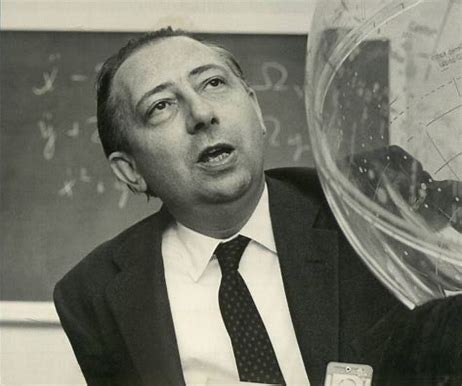
\includegraphics[scale=0.2]{wigner}
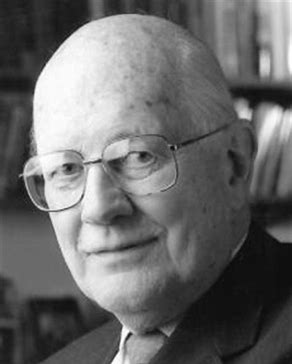
\includegraphics[scale=0.21]{seitz}
\end{figure}
\ech
\end{frame}
  
\begin{frame}\frametitle{\bch 小群的表示\ech}
  \bch
  因为小群的元素保持4-动量不变,所以变换后的态可以写成$|p^{\prime},\zeta\rangle$的线性组合。
  \be
  U(\Gamma) |p^{\prime},\zeta\rangle = \sum_{\zeta^\prime} D_{\zeta^\prime \zeta} (\Gamma)|p^{\prime},\zeta^\prime\rangle
  \ee
  因此,$D_{\zeta^\prime \zeta}$是$\Gamma$的一个不可约表示。对于下面的情况,我们把不可约表示求出来
  \begin{itemize}
  \item massive particles,
  \item massless particles.
  \end{itemize}
  \ech
\end{frame}
\begin{frame}\frametitle{\bch massive particles\ech}
  \bch
  先考虑最简单的情况,粒子静止,即$p^{\prime}_0 = m, p_i^\prime = 0$,这时什么是保持$p^\prime$不变的变换?显然,三维空间的旋转。令$\zeta$是自旋,故矩阵为
  \be
  D(R) = D^{(s)}(R(\vec{\theta})) = \exp(-i\vec{\theta}\cdot \vec{s})
  \ee
  例如,对于自旋$1/2$,有
  \be
  D^{(1/2)} = \exp\left(-i\vec{\theta}\cdot \frac{\vec{\sigma}}{2}\right)
  \ee
  其中$\vec{\sigma}$是三个Pauli矩阵。
  \ech
\end{frame}
\begin{frame}\frametitle{\bch Lorentz Boost\ech}
  \bch
  上面我们在静止系下获得了小群的表示论,现在我们试图在相对粒子运动的参考系下找表示论,由于两个参考系之间差一个Lorentz Boost $L(p)$,我们用以下的步骤来找运动参考系的表示论。
  \begin{itemize}
  \item 首先, reboost。将$L(p)^{-1}$作用在运动参考系的态上。
  \item 在静止参考系变换。
  \item 再boost 回来,作用$L(p)$在变换好的态上。
  \end{itemize}
  因此$R(P,\Lambda) = L(\Lambda p)^{-1} \Lambda L(p)$就是运动参考系的小群。这又被叫做 Wigner 转动。
  \ech
\end{frame}
\begin{frame}\frametitle{\bch Massless Particles \ech}
  \bch
  无质量的粒子不可能静止下来,所以上面的方法就不管用了。对于无质量粒子有
  \be
  p^{\prime 2} =0
  \ee
  假设3-动量沿着z轴方向,则
  \be
  p_3^{\prime} = p_0^{\prime}
  \ee
  取$p_0^\prime =1$,那么这种情况的小群为$\Lambda_t R_z(\theta)$,其中
  \be
  \Lambda_t =
  \begin{pmatrix}
    1&0&0 \\
    0&1&0\\
    \lambda_{31} &\lambda_{32} & 1
  \end{pmatrix}
  \ee
  但是,如果为了使系统具有分立的自旋(因为观测),必须有
  \be
  D(\Lambda_t) \equiv 1 ,\spa D(R_z(2\pi)) = \pm 1
  \ee
  \ech
\end{frame}
\begin{frame}\frametitle{\bch $R_z(\theta)$\ech}
  \bch
  现在,回忆我们熟悉的$SO(2)$,因为$SO(2)$群是阿贝尔群,所以它只有一维不可约表示,所以
  \be
  D_{\lambda^\prime \lambda}(\Gamma) = \delta_{\lambda\lambda^\prime} e^{-i\lambda\theta}
  \ee
  因为$D(R_z(2\pi))=\pm 1$,这就意味着$\lambda$是一个整数或者半整数。
  \ech
\end{frame}
\begin{frame}\frametitle{\bch 无质量粒子的特性\ech}
  \bch
  如果我们再考虑宇称的话,我们会发现无质量粒子的helicity 只能取$\pm \lambda$。
  \begin{itemize}
  \item 光子,自旋为1,只有$\pm 1$的helicity。
  \item 胶子,自旋为1,只有$\pm 1$的helicity。
  \item 引力子,自旋为2,$\pm 2$。
  \item 中微子,自旋1/2,以前认为是无质量粒子,有两种helicity。
  \end{itemize}
  \ech
\end{frame}


  

\end{document}
